\subsubsection{Activity Diagram - Quản lý phân quyền}

\begin{figure}[H]
    \centering
    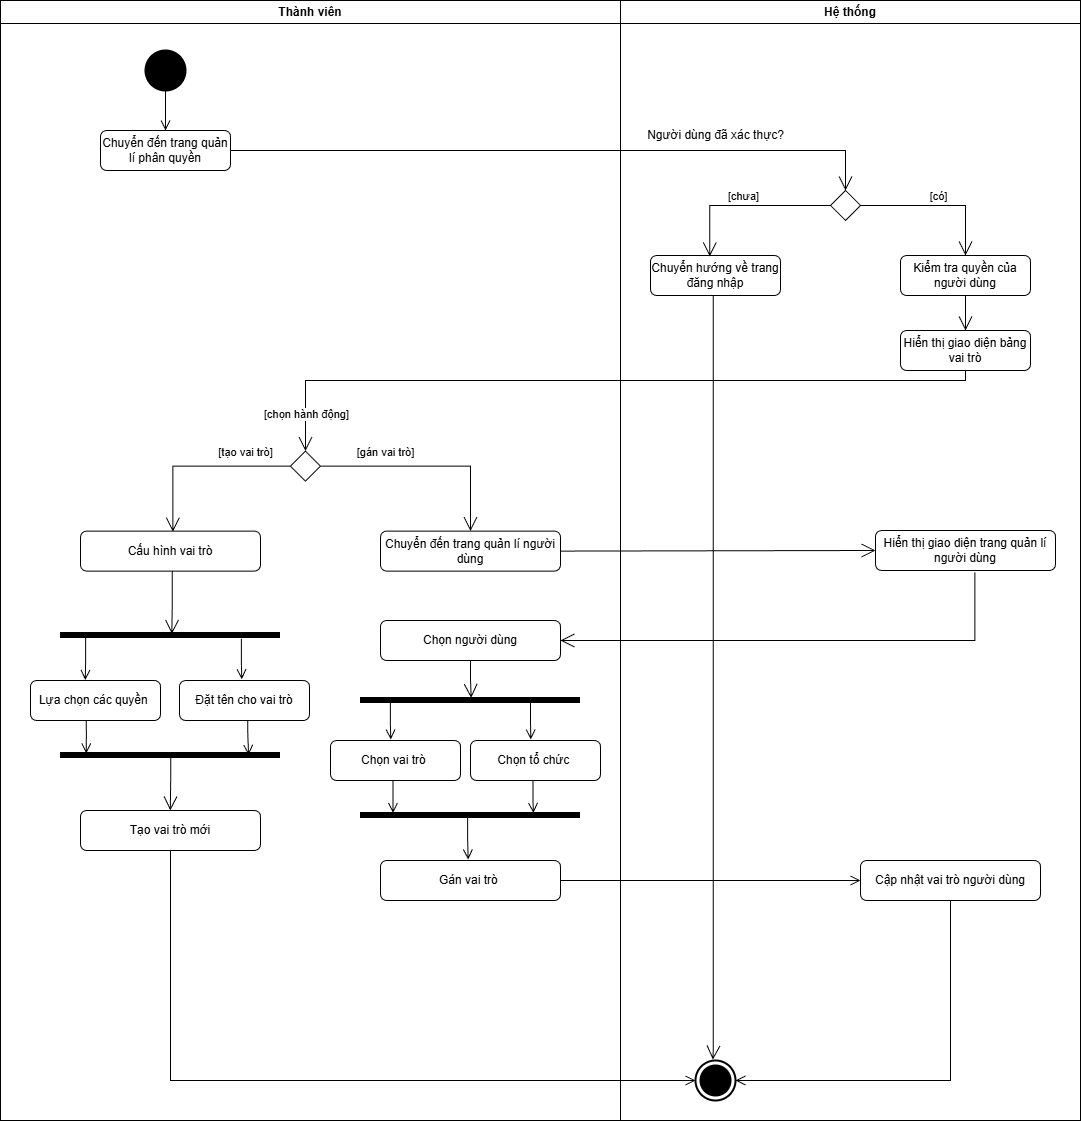
\includegraphics[width=1.0\textwidth]{Images/activity-diagram/authorization-activity.drawio.png} 
    \vspace{0.5cm}
    \caption{Activity Diagram - Quản lý phân quyền}
    \label{fig:act_auth}
\end{figure}
Biểu đồ hoạt động (Activity Diagram) tại Hình \ref{fig:act_auth} mô tả chi tiết quy trình nghiệp vụ quản lý phân quyền, bao gồm các bước kiểm soát truy cập và hai luồng chức năng chính: Cấu hình vai trò mới và Gán vai trò cho người dùng.
Quy trình được chia thành hai làn xử lý (\textit{Swimlanes}) là \textbf{Thành viên} (Quản trị viên) và \textbf{Hệ thống}, với các bước xử lý cụ thể như sau:

\paragraph{Kiểm soát truy cập ban đầu}
Khi người dùng truy cập vào trang quản lý phân quyền, hệ thống thực hiện lớp bảo mật đầu tiên:
\begin{itemize}
    \item \textbf{Kiểm tra xác thực:} Hệ thống xác minh xem phiên làm việc của người dùng có hợp lệ không.
    \item \textbf{Điều hướng:} 
    \begin{itemize}
        \item Nếu chưa xác thực: Hệ thống tự động chuyển hướng về trang Đăng nhập.
        \item Nếu đã xác thực: Hệ thống tiếp tục kiểm tra quyền hạn cụ thể của người dùng trước khi hiển thị giao diện bảng danh sách vai trò.
    \end{itemize}
\end{itemize}

\paragraph{Các luồng nghiệp vụ chính}
Tại giao diện quản lý, quản trị viên có thể lựa chọn một trong hai hành động, dẫn đến hai nhánh xử lý khác nhau:

\begin{itemize}
    \item \textbf{Nhánh 1: Tạo vai trò mới (Create Role)}
    Quy trình này sử dụng cơ chế xử lý song song (\textit{Parallel Processing}) để tối ưu hóa thao tác nhập liệu:
    \begin{enumerate}
        \item Quản trị viên vào màn hình cấu hình vai trò.
        \item Hệ thống cho phép thực hiện đồng thời hai tác vụ: \textit{Lựa chọn các quyền hạn (Permissions)} và \textit{Đặt tên cho vai trò}.
        \item Sau khi hoàn tất cả hai thông tin trên, hệ thống tổng hợp và tạo vai trò mới trong cơ sở dữ liệu.
    \end{enumerate}

    \item \textbf{Nhánh 2: Gán vai trò cho người dùng (Assign Role)}
    Đây là quy trình cấp quyền truy cập cụ thể cho từng thành viên:
    \begin{enumerate}
        \item Hệ thống chuyển hướng và hiển thị danh sách người dùng.
        \item Quản trị viên chọn một tài khoản người dùng cụ thể.
        \item Tương tự như quy trình tạo vai trò, hệ thống yêu cầu xác định song song hai yếu tố: \textit{Vai trò cần gán} và \textit{Tổ chức áp dụng} (Scope). Điều này đảm bảo tính linh hoạt của mô hình RBAC, cho phép một người dùng có thể giữ các vai trò khác nhau tại các tổ chức khác nhau.
        \item Cuối cùng, hệ thống cập nhật thông tin phân quyền vào cơ sở dữ liệu và kết thúc quy trình.
    \end{enumerate}
\end{itemize}